\documentclass[25pt]{sciposter}

\usepackage[T1]{fontenc}
\usepackage[utf8]{inputenc}

\usepackage{amsthm}

\usepackage[dvipsnames,usenames,svgnames,table]{xcolor} 
\usepackage{lipsum}
\usepackage{epsfig}
\usepackage{amsmath}
\usepackage{amssymb}
\usepackage[german]{babel}
\usepackage{geometry}
\usepackage{multicol}
\usepackage{graphicx}
\usepackage{tikz}
\usepackage{wrapfig}
\usepackage{gensymb}
\usepackage[utf8]{inputenc}
\usepackage{empheq}
\usepackage{mathtools}

\usepackage{pgfplots}
\pgfplotsset{width=11cm,compat=1.9}


% for nice tableas
\usepackage{booktabs}

\graphicspath{ {img/} }

\geometry{
 landscape,
 a1paper,
 left=5mm,
 right=50mm,
 top=5mm,
 bottom=50mm,
 }



%BEGIN LISTINGDEF



\usepackage{listings}
\usepackage{sourcecodepro}
\definecolor{listing-background}{rgb}{0.97,0.97,0.97}
\definecolor{listing-rule}{HTML}{B3B2B3}
\definecolor{listing-numbers}{HTML}{B3B2B3}
\definecolor{listing-text-color}{HTML}{000000}
\definecolor{listing-keyword}{HTML}{435489}
\definecolor{listing-identifier}{HTML}{435489}
\definecolor{listing-string}{HTML}{00999a}
\definecolor{listing-comment}{HTML}{8e8e8e}
\definecolor{listing-javadoc-comment}{HTML}{006CA9}

\lstdefinestyle{eisvogellistingstyle}{
	language=java,
	numbers=left,
	backgroundcolor=\color{listing-background},
	basicstyle=\color{listing-text-color}\small\ttfamily{}, % print whole listing small
	xleftmargin=0.8em, % 2.8 with line numbers
	breaklines=true,
	frame=single,
	framesep=0.6mm,
	rulecolor=\color{listing-rule},
	frameround=ffff,
	framexleftmargin=0.4em, % 2.4 with line numbers | 0.4 without them
	tabsize=4, %width of tabs
	numberstyle=\color{listing-numbers},
	aboveskip=1.0em,
	keywordstyle=\color{listing-keyword}\bfseries, % underlined bold black keywords
	classoffset=0,
	sensitive=true,
	identifierstyle=\color{listing-identifier}, % nothing happens
	commentstyle=\color{listing-comment}, % white comments
	morecomment=[s][\color{listing-javadoc-comment}]{/**}{*/},
	stringstyle=\color{listing-string}, % typewriter type for strings
	showstringspaces=false, % no special string spaces
	escapeinside={/*@}{@*/}, % for comments
	literate=
	{á}{{\'a}}1 {é}{{\'e}}1 {í}{{\'i}}1 {ó}{{\'o}}1 {ú}{{\'u}}1
	{Á}{{\'A}}1 {É}{{\'E}}1 {Í}{{\'I}}1 {Ó}{{\'O}}1 {Ú}{{\'U}}1
	{à}{{\`a}}1 {è}{{\'e}}1 {ì}{{\`i}}1 {ò}{{\`o}}1 {ù}{{\`u}}1
	{À}{{\`A}}1 {È}{{\'E}}1 {Ì}{{\`I}}1 {Ò}{{\`O}}1 {Ù}{{\`U}}1
	{ä}{{\"a}}1 {ë}{{\"e}}1 {ï}{{\"i}}1 {ö}{{\"o}}1 {ü}{{\"u}}1
	{Ä}{{\"A}}1 {Ë}{{\"E}}1 {Ï}{{\"I}}1 {Ö}{{\"O}}1 {Ü}{{\"U}}1
	{â}{{\^a}}1 {ê}{{\^e}}1 {î}{{\^i}}1 {ô}{{\^o}}1 {û}{{\^u}}1
	{Â}{{\^A}}1 {Ê}{{\^E}}1 {Î}{{\^I}}1 {Ô}{{\^O}}1 {Û}{{\^U}}1
	{œ}{{\oe}}1 {Œ}{{\OE}}1 {æ}{{\ae}}1 {Æ}{{\AE}}1 {ß}{{\ss}}1
	{ç}{{\c c}}1 {Ç}{{\c C}}1 {ø}{{\o}}1 {å}{{\r a}}1 {Å}{{\r A}}1
	{€}{{\EUR}}1 {£}{{\pounds}}1 {«}{{\guillemotleft}}1
	{»}{{\guillemotright}}1 {ñ}{{\~n}}1 {Ñ}{{\~N}}1 {¿}{{?`}}1
}
\lstset{style=eisvogellistingstyle}



%END LISTINGDEF


\newcommand*\widefbox[1]{\fbox{\hspace{2em}#1\hspace{2em}}}
\newcommand{\limm}{\lim\limits_{n \to \infty}}
\newcommand{\limx}[1]{\lim\limits_{x \to #1}}
\newlength\dlf  % Define a new measure, dlf
\newcommand\alignedbox[2]{
% Argument #1 = before & if there were no box (lhs)
% Argument #2 = after & if there were no box (rhs)
&  % Alignment sign of the line
{
\settowidth\dlf{$\displaystyle #1$}
    % The width of \dlf is the width of the lhs, with a displaystyle font
\addtolength\dlf{\fboxsep+\fboxrule}
    % Add to it the distance to the box, and the width of the line of the box
\hspace{-\dlf}
    % Move everything dlf units to the left, so that & #1 #2 is aligned under #1 & #2
\boxed{#1 #2}
    % Put a box around lhs and rhs
}
}
\usepackage{graphicx,url}

%BEGIN TITLE
\title{\huge{Analysis 1}}

\author{\large{David Zollikofer}}
%END TITLE

\usepackage{palatino}

% begin custom commands
\newcommand{\Q}{\mathbb{Q}}
\newcommand{\R}{\mathbb{R}}
\newcommand{\N}{\mathbb{N}}
%\newcommand{\cos}{\operatorname{cos}}
%\newcommand{\sin}{\operatorname{sin}}
%\newcommand{\exp}{\operatorname{exp}}

\newtheorem{thm}{Thm}[section]



\usepackage[framemethod=TikZ]{mdframed}
\newenvironment{method}[1]{\begin{mdframed}[backgroundcolor=blue!10,innertopmargin=15pt, innerbottommargin=15pt, nobreak=true]
		\textbf{#1 }
	}
	{ 
	\end{mdframed}
}
\usepackage{todonotes}
\newcommand{\TODO}[1]{\todo[inline]{\Large TODO:  #1}}





\DeclarePairedDelimiter\abs{\left|}{\right|}%
\DeclarePairedDelimiter\norm{\lVert}{\rVert}%


\setlength\abovedisplayskip{0pt}


% end custom commands

\begin{document}

\fontfamily{ppl}\selectfont



\maketitle


\begin{multicols}{3}


\section{Einführung}
\begin{method}{Ordnungsvollständigkeit}
Unterscheidet $\R$ von $\Q$. Für $A,B$ nichtleere Teilmengen von $\R$ mit $$\forall a\in A \land \forall b \in B \implies a \leq b$$
Dann gibt es $c \in \R$ mit $\forall a \in A : a \leq c$ und $\forall b \in B : c \leq b$
\end{method}


\begin{method}{Archimedisches Prinzip}
Korollar von Ordnungsvollständigkeit. Sei $x\in \R$ mit $x>0$ und $y \in \R$, dann gibt es $n\in \N$ mit $y \leq nx$
\end{method}

\subsection*{Youngsche Ungleichung}
$\forall \epsilon > 0 , \forall x,y\in \R$ gilt: $2 |xy| \leq \epsilon x^2 + \frac{1}{\epsilon} y^2$. Beweis per Expansion von $\left( \sqrt{\epsilon} |x| - \frac{1}{\sqrt{\epsilon}} |y| \right) ^2 \geq 0$

\begin{method}{Existenz des Supremums}
Sei $A \subset \R$, $A \not = \varnothing$. Sei $A$ nach oben beschränkt, dann gibt es eine kleinste obere Schranke von $A$, $c = \sup A$, genannt Supremum von $A$. Um dies zu Beweisen nutzt man die Ordnungsvollständigkeit und definiert $B$ als die Menge der oberen Schranken.
\end{method}
\textbf{Beispiel (Sup \& Inf finden)} Sei $M = \{ \frac{|x|}{1 + |x|} : x \in \mathbb{R}\}$. \\ \textsc{Infinum:} Weil alle Elemente positiv sind ist von unten durch 0 beschränkt. Falls $x = 0$, folgt $\frac{|0|}{|0|+1} =0$ womit $\min{M} = \inf{M} = 0$. \\
\textsc{Supremum:} Für alle $x$ gilt $|x| + 1 > |x|$ somit $\frac{|x|}{|x|+1} < 1$. Somit gilt sicher $\sup M \leq 1$. \\
Nach Archimedes: $\forall \epsilon > 0,\exists n_0 : 1/n \leq \epsilon \ \forall n \geq n_0$
$$\frac{n}{n+1} = \frac{1}{1 + \frac{1}{n}} =\geq \frac{1}{1 + \epsilon} = 1 - \frac{\epsilon}{1 + \epsilon}$$
Wir erreichen $1$ sicher nie da sonst $1 = 0$, aber wir können beliebig nahe kommen. Somit $\sup M = 1$ aber $\neg \exists \max M$

\begin{method}{Cauchy Schwarz}
$\forall x,y\in \R^n$ gilt $|\langle x,y\rangle| \leq ||x||\cdot||y||$.
\end{method}


\begin{method}{Komplexe Zahlen}\\
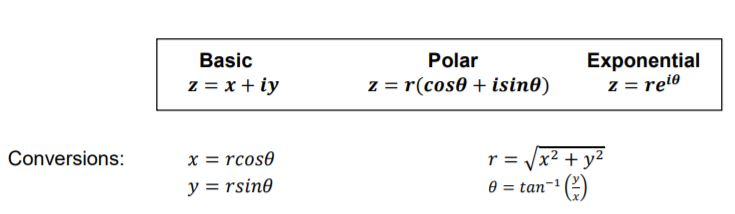
\includegraphics[scale=1.4]{complex.jpg}\\
\textsc{Division:} Es gilt $z^{-1} = \frac{\bar{z}}{||z||^2}$ wenn $z \not = 0$\\
\textsc{Polarform} Wenn \begin{align*}
z_1 &= r_1(\cos(\theta_1) + i\sin(\theta_1))\\
z_2 &= r_2(\cos(\theta_2) + i\sin(\theta_2))
\end{align*}
dann gilt: 
\begin{align*}
z_1 \cdot z_2 &= r_1 \cdot r_2 \left(\cos(\theta_1 + \theta_2) + i\sin(\theta_1 + \theta_2)\right)\\
\frac{z_1}{z_2} &= \frac{r_1}{r_2}\left(\cos(\theta_1 - \theta_2) + i\sin(\theta_1 - \theta_2)\right)
\end{align*}
Zudem folgt durch Induktion:
$$z^n = r^n (\cos(n\theta) + i \sin(n \theta))$$
\end{method}





% -------------------------- Folgen --------------------------

\section{Folgen}

\begin{method}{Definition Konvergenz}
Folge $a_n$ is konvergent, falls $\exists l \in \mathbb{R}$ so dass $\forall \epsilon > 0$ die Menge $\{n \in \mathbb{N}^+: a_n \not \in (l-\epsilon, l + \epsilon)\}$ endlich ist. \\
Äquivalent: $\forall \epsilon > 0 \ \exists N \in \N $ so dass $ \forall n \geq N$ gilt $|a_n - l|< \epsilon$.
\end{method}

\textbf{Beispiel (Konvergenz mit Definition)}: 
Beweise dass $\limm \frac{3n^2 + 4}{2n^2 + 1} = \frac{3}{2}$. Sei $\epsilon > 0$. Dann muss gelten $|a_n - a | < \epsilon$. Somit $\left| \frac{3n^2 + 4}{2n^2 + 1} -  \frac{3}{2}\right| = \left| \frac{6n^2 + 8 - 6n^2 -3}{4n^2 + 2} \right| = \frac{5}{4n^2 + 2} < \epsilon$. Gibt $4n^2 + 2 > \frac{5}{\epsilon}$, äquiv zu $n > \sqrt{\frac{5}{4 \epsilon} - \frac{1}{2}}$. Wir definieren $N = \lfloor \sqrt{\frac{5}{4 \epsilon} - \frac{1}{2}} \rfloor$. Nun gilt $\forall n \geq N : |a_n - a | < \epsilon$.




\begin{method}{Rechnen mit Grenzwerten} $(a_n)_n$ und $(b_n)_n$ konvergent mit GW $a,b$. Dann gilt:
	\begin{itemize}
		\item $\lim \limits_{n \to \infty} (a_n + b_n) = a + b$	
		\item $\lim \limits_{n \to \infty} (a_n \cdot b_n) = a \cdot b$
		\item  Falls $b_n, b \not = 0$, so gilt $\lim \limits_{n \to \infty} \frac{a_n}{b_n} = \frac{a}{b}$
		\item Falls $a_n \leq b_n$ $\forall n \in \mathbb{N}$, so gilt $a \leq b$
	\end{itemize}
\end{method}

\textbf{Beispiel (Rechnen mit Grenzwerten)}: 
\begin{itemize}
	\item $\limm  \frac{(\frac{1}{n} + n^2 )^3}{1 + n^6} = \limm \frac{n^6}{n^6} \frac{(\frac{1}{n^3} + 1 )^3}{\frac{1}{n^6} + 1} = \limm \frac{(\frac{1}{n^3} + 1 )^3}{\frac{1}{n^6} + 1} = 1$
	
	\item $\limm \sqrt{n} (\sqrt{n + 2} - \sqrt{n}) \stackrel{\text{Wurzeltrick}}{=} \limm \frac{2 \sqrt{2}}{\sqrt{n+2} + \sqrt{n}} = \limm  \frac{2}{\sqrt{1 + \frac{2}{n}} + 1} = 1$
\end{itemize}

\begin{method}{Satz von Weierstrass}
	Wenn $a_n$ nach oben (nach unten) konvergent ist und monoton wachsend (fallend), dann ist $a_n$ konvergent.
\end{method}

\textbf{Beispiel (Induktive Folge mit Weierstrass)}: 
Beachte $a_0 = 0$, $a_{n+1} = \left(\frac{a_n}{2}\right)^2 + 1$. \textsc{Monotonie:} Anstatt $a_{n+1} > a_{n}$ zeigen wir $a_{n+1} - a_{n} > 0$:
$$a_{n+1} - a_{n} = \frac{a_n ^2}{4} + 1 - a_n = \frac{a_n ^2 -4a_n + 4}{4} = \frac{(2-a_n)^2}{4} \geq 0$$
\textsc{Beschränktheit:} ($\leq 2$) per Induktion. Für $n=0$, $a_0 = 0 \leq 2 \checkmark$. Schritt: $a_{n+1} = \frac{a_n ^2}{4} + 1 \stackrel{\text{I.H.}}{\leq} \frac{2^2}{4} +1 = 2 \checkmark$. Nach Weierstrass konvergent. mit $a = \frac{a^2}{4} + 1 \implies a = 2$ als GW.


\begin{method}{Sandwich Theorem}
Seien $b_n \leq a_n \leq c_n$. Falls $b_n$ und $c_n$ konvergent sind mit $\lim \limits_{n \to \infty } b_n = \lim \limits_{n \to \infty } c_n = L$, so ist $a_n$ auch konv. mit $\lim \limits_{n \to \infty } a_n = L$
\end{method}
\textbf{Beweis (Sandwich Theorem)}: 
Da $b_n$, $c_n$ konvergent mit GW $L$:
$$\forall \epsilon > 0 \exists N_1 : \forall n \geq N_1 : L-\epsilon < b_n + \epsilon$$
Analog  $ \exists N_2$, setze $N = \max\{N_1, N_2\}$, dann gilt $\forall \epsilon > 0 \exists N$:
$$L-\epsilon < b_n \leq a_n \leq c_n < L + \epsilon \implies L - \epsilon < a_n < L + \epsilon$$


\textbf{Beispiel (Sandwich)}
$\limm \frac{n + \cos(n)}{n^2 -1}$. Wenn es absolut konv. dann auch absolut. Sicher gilt somit : $0 \leq \left|\frac{n + \cos(n)}{n^2 -1}\right|$ Nun schätzen wir nach oben ab: $\left|\frac{n + \cos(n)}{n^2 -1}\right| \leq \frac{n+1}{n^2 - 1} = \frac{n+1}{(n+1)(n-1)} = \frac{1}{n-1}$. Es gilt $\limm \frac{1}{n-1} = 0$, somit gilt $\limm \left|\frac{n + \cos(n)}{n^2 -1}\right| = 0$. (da Sandwich)

\begin{method}{Bernoulli - de l’Hospital}
	Wenn wir zwei differenzierbare Funktionen $f$ $g$ haben mit $g'(a)\not = 0$ dann gilt falls:
	\begin{itemize}
		\item entweder $\lim_{x \to a} f(x) = \lim_{x \to a} g(x) = 0 $
		\item oder $\lim_{x \to a} f(x) = \lim_{x \to a} g(x) = \infty $
	\end{itemize}
dann gilt:
\begin{equation*}
	\lim_{x \to a} \frac{f(x)}{g(x)} = 	\lim_{x \to a} \frac{f'(x)}{g'(x)}
\end{equation*}
\end{method}
\begin{itemize}
	\item \textbf{Typ 1: $\frac{0}{0}$ oder $\frac{\infty}{\infty}$}\\
	\textit{Beispiele:}
	\begin{itemize}
		\item $\limx{0^+}\sqrt{\frac{1- \cos(x)}{2x}} = \sqrt{\limx{0^+}\frac{1- \cos(x)}{2x}} =  \sqrt{\limx{0^+}\frac{\sin(x)}{2}} = 0$, wobei wir die Stetigkeit nutzten.
		\item $\limx{0^+} \frac{e^{-\frac{1}{x}}}{x} = \limx{0^+} \frac{\frac{1}{x}}{e^{-\frac{1}{x}}} = \frac{-\frac{1}{x^2}}{-\frac{1}{x^2}e^{\frac{1}{x}}} = \limx{0^+} e^{- \frac{1}{x}} = 0$
		\item $\limx{0} \frac{\sin(\pi\cos(x))}{x\sin(x)} = \limx{0} \frac{-\sin(x)\pi\cos(\pi\cos(x))}{x\cos(x)+\sin(x)} = \limx{0} \frac{-\pi\cos(\pi\cos(x))}{\frac{x}{\sin(x)}\cos(x)+1} = \limx{0} \frac{-\pi\cos(\pi\cos(x))}{1+1} = \frac{-\pi\cos(\pi)}{2} = \frac{\pi}{2}$
	\end{itemize}
	\item \textbf{Typ 2: $0 \cdot \infty$} Wenn wir einen Grenzwert wie $\lim\limits_{x \to a} f(x)g(x)$ haben dann können wir den umformen in:
\begin{align*}
	\lim_{x \to a}f(x) g(x) &= \lim_{x\to a} \frac{f(x)}{\frac{1}{g(x)}}\\
		\lim_{x \to a}f(x) g(x) &= \lim_{x\to a} \frac{g(x)}{\frac{1}{f(x)}}
\end{align*}
\textit{Beispiele:}
\begin{itemize}
	\item $\limx{0^+} x\ln(x) = \limx{0^+} \frac{\ln(x)}{\frac{1}{x}} = \limx{0^+} \frac{\frac{1}{x}}{-\frac{1}{x^2}} = \limx{0^+} -\frac{x^2}{x} = 0$
	\item $\limx{\frac{\pi}{2}^-} \left( \tan(x) - \frac{1}{\cos(x)} \right) = \limx{\frac{\pi}{2}^-} \left(\frac{\sin(x)}{\cos(x)}- \frac{1}{\cos(x)} \right) = \limx{\frac{\pi}{2}^-} \frac{\sin(x) -1}{\cos(x)} = \limx{\frac{\pi}{2}^-} \frac{\cos(x)}{-\sin(x)} = \frac{\cos(\frac{\pi}{2})}{-\sin(\frac{\pi}{2})} = \frac{0}{-1} = 0$
	\item $\limx{+ \infty} x \left( \sqrt[x]{e} -1 \right) = \limx{+ \infty} \frac{e^{-\frac{1}{x}}-1}{\frac{1}{x}} = \limx{+ \infty} \frac{\frac{1}{-x^2}e^{-\frac{1}{x}}}{\frac{1}{-x^2}} = \limx{+ \infty} e^{-\frac{1}{x}} = 0$
\end{itemize}
	
	
	\item \textbf{Typ 3: $f(x)^{g(x)}$} Wenn wir Grenzwerte des Types $ \limx{a} f(x)^{g(x)}$ haben, dann schreiben wir es wie folgt:
	\begin{align*}
		\limx{a} f(x)^{g(x)} &= \limx{a} e^{\ln(f(x))\cdot g(x)} = e^{\limx{a} \ln(f(x))\cdot g(x)}
	\end{align*}
	\textit{Beispiele:}
	\begin{itemize}
		\item $\limx{0^+} x^{\sin(x)} = e^{\limx{0^+} \sin(x)\ln(x)}$. Nun schauen wir den Exponenten an: $\limx{0^+} \sin(x)\ln(x) = \limx{0^+} \frac{\ln(x)}{\frac{1}{\sin(x)}} = \limx{0^+} \frac{\frac{1}{x}}{\frac{-\cos(x)}{\sin^2(x)}} = \limx{0^+} \frac{\sin^2(x)}{- x\cos(x)} = \limx{0^+} -\frac{\sin(x)}{x} \cdot\frac{\sin(x)}{\cos(c)} = 1 \cdot 0 = 0$. Wir haben somit $e^0 = 1$.
		\item $\limx{0^+} \left( \sqrt{x^2 + 1} \right)^{\frac{1}{\sin^2(x)}} = e^{\left(\limx{0^+} \frac{\ln(\sqrt{x^2 + 1})}{\sin^2(x)} \right)}$. Nun schauen wir den Exponenten an: $\limx{0^+} \frac{\ln(\sqrt{x^2 + 1})}{\sin^2(x)} = \limx{0^+} \frac{\ln(x^2 + 1)}{2\sin^2(x)} = \limx{0^+} \frac{\ln(x^2 + 1)}{2\sin^2(x)} = \limx{0^+} \frac{\frac{1}{x^2+1}\cdot 2x}{4\sin(x)\cos(x)} = \limx{0^+} \frac{1}{2}\cdot \frac{x}{\sin(x)} \cdot \frac{1}{(x^2 + 1) \cos(x)} = \frac{1}{2}$. Somit haben wir somit $e^{\frac{1}{2}}$.
	\end{itemize}
\end{itemize}



\begin{method}{Cauchy Kriterium}
	Die Folge $(a_n)_n$ ist genau dann konvergent, falls $\forall  \epsilon > 0 \ \exists N \geq 1 \text{ so dass } |a_n - a_m| < \epsilon \quad \forall n,m \geq N$
\end{method}

\TODO{Beweis von Cauchy}

\textbf{Beispiel (Cauchy Kriterium)}
Sei $a_n = \frac{n-1}{2n}$ eine Folge. Wir versuchen Konvergenz mittels Cauchy zu zeigen:\\
$|a_n - a_m| = |\frac{n-1}{2n} - \frac{m-1}{2m}| = |\frac{nm-m-nm+n}{2nm}| = |\frac{n-m}{2nm}| = \frac{1}{2n} - \frac{1}{2m} \stackrel{m\geq n}{\leq} \frac{1}{2n} < \epsilon$. Für alle $n \geq N = \lceil \frac{1}{2\epsilon} \rceil$ haben wir $|a_n - a_m| < \epsilon$. Nach Cauchy ist $a_n$ somit konvergent.

\begin{method}{Satz von Bolzano Weierstrass}
	Jede beschränkte Folge besitzt eine konvergente Teilfolge.
\end{method}


% -------------------------- Reihen --------------------------

\section{Reihen}

\begin{method}{Konvergenz mit Definition} Eine Reihe konvergiert wenn der Grenzwert der Partialsummen existiert:
	$$\sum_{n=0}^{\infty} a_n  = \lim\limits_{N\to\infty} S_n = \lim\limits_{N\to\infty} \sum_{n=0}^{\infty} a_n$$
\end{method}

\textbf{Beispiel (Konvergenz mit Definition)}
\begin{itemize}
	\item $\sum_{n = 0}^{\infty} \frac{1}{n(n+1)} = \frac{1}{n} - \frac{1}{n+1}$. Es gilt somit $S_n = 1 - \frac{1}{2} + \frac{1}{2} - \frac{1}{3} \ldots - \frac{1}{n+1}$ Somit $S_n = 1-\frac{1}{n+1}$. Es gilt $\limm S_n = \limm 1 - \frac{1}{n+1} = 1$, somit ist die Reihe konvergent mit Grenzwert 1.
	\item $\sum_{n = 0}^{\infty} \frac{1}{\sqrt{n} + \sqrt{n+1}} $ Zuerst nutzen wir den Wurzeltrick: $\frac{1}{\sqrt{n} + \sqrt{n+1}} = \sqrt{n+1} - \sqrt{n}$. Wir bemerken $S_n = 1 - 0 + \sqrt{2} - 1 \ldots + \sqrt{n+1} - \sqrt{n} = \sqrt{n+1}$. Da aber $\limm S_n =  \limm \sqrt{n+1} = \infty$ divergiert die Reihe.
\end{itemize}

\begin{method}{Geometrische Reihen}
	Für geometrische Reihen gilt:
	$$\sum _{k=0}^{n-1}ar^{k}=a\left({\frac {1-r^{n}}{1-r}}\right)$$
	\textit{Beweis:}{\begin{align*}s&=a+ar+ar^{2}+ar^{3}+\cdots +ar^{n-1},\\rs&=ar+ar^{2}+ar^{3}+ar^{4}+\cdots +ar^{n},\\s-rs&=a-ar^{n},\\s(1-r)&=a(1-r^{n}),\end{align*}}
\end{method}

\begin{method}{Konvergenz mit $\lim\limits_{n \to \infty } a_n = 0$}
$$\sum_{n=0}^{\infty} a_0 \text{ konvergiert } \implies \lim\limits_{n \to \infty } a_n = 0 $$
\end{method}

\textbf{Beweis (Nullfolge)} Wenn $\sum_{n = 0}^{\infty} a_n$ konvergent ist, dann ist $\limm a_n = 0$.
Es gilt $a_N = S_N - S_{N-1}$. Somit $\limm a_n = \limm (S_n - S_{n-1}) = \limm S_n - \limm S_{n-1} = S-S = 0$

\begin{method}{Majorantenkriterium}
	Fall $a_n \geq b_n \forall n \geq n_0$ für ein $n_0$. Dann gilt $\sum_n a_n \text{ konvergiert } \implies \sum_{n} b_n$ konvergiert.
\end{method}

\begin{method}{Minorantenkriterium}
	Fall $a_n \geq b_n \forall n \geq n_0$ für ein $n_0$. Dann gilt $\sum_n b_n \text{ divergiert } \implies \sum_{n} a_n$ divergiert.
\end{method}




\begin{method}{Quotientenkriterium}
	Sei $a_n \not = 0$, dann gilt:
	\begin{itemize}
		\item $\lim\limits_{n \to \infty} |\frac{a_{n+1}}{a_n}|> 1 \implies \sum_{n} a_n$ divergiert. 
		\item $\lim\limits_{n \to \infty} |\frac{a_{n+1}}{a_n}|< 1 \implies \sum_{n} a_n$ konvergiert. 
		\item $\lim\limits_{n \to \infty} |\frac{a_{n+1}}{a_n}|=  1 \implies $ Kriterium versagt.
	\end{itemize}
\end{method}

\textbf{Beweis (Quotientenkriterium)} Angenommen $c_n = \sup\{ \frac{|a_{k+1}|}{|a_{k}|} : k \geq n \}$. Dann wenn beschränkt: $\limsup_{n\to \infty} \frac{|a_{n+1}|}{|a_{n}|} = \limm c_n$. Angenommen wir haben $q$ so dass $\limm c_n < q < 1$. Sei $N \geq 1$ so dass $c_N \leq q < 1$ woraus $\frac{|a_{k+1}|}{|a_k|} \leq q$ $\implies |a_{k+1}| \leq q |a_k|$. Für $j\geq 1$ folgt: $|a_{N+j}|\leq q|a_{N+j-1}| \leq \ldots \leq q^j |a_N| = q^{N+j} \frac{|a_N|}{q^N}$. Somit gilt: $|a_n| \leq q^n \frac{|a_N|}{q^N}$ und wir haben eine Majorante.

\textbf{Beispiel (Quotientenkriterium)}

\begin{itemize}
	\item $\sum_{n = 1}^\infty \frac{4^n}{n!}$. $\limm \frac{|a_{n+1}|}{|a_n|} = \limm \frac{4^{n+1} n!}{4^n (n+1)!} = \limm \frac{4}{n+1} = 0 < 1$. Konvergent $\checkmark$
	
	\item $\sum_{n = 1}^\infty \frac{n^n}{(2n)!!}$.  $\limm \frac{|a_{n+1}|}{|a_n|}  = \frac{(n+1)^{n+1}}{(2n+2)!!} \frac{(2n)!!}{n^n} = \limm \frac{(n+1)^{n+1}}{n^n} \frac{(2n)!!}{(2n+2)(2n)!!} = \limm \frac{1}{2} \left( \frac{n+1}{n} \right)^n = \frac{e}{2}>1$. Somit divergent.
\end{itemize}





\begin{method}{Wurzelkriterium}
	\begin{itemize}
		\item $\lim\limits_{n \to \infty} \sqrt[n]{|a_n|}>1 \implies \sum_{n} a_n $ divergiert
		\item $\lim\limits_{n \to \infty} \sqrt[n]{|a_n|}<1 \implies \sum_{n} a_n $ konvergiert
		\item $\lim\limits_{n \to \infty} \sqrt[n]{|a_n|}=1 \implies $ Kriterium versagt
	\end{itemize}
\end{method}

\textbf{Beispiel (Wurzelkriterium)}
\begin{itemize}
	\item $\sum_{n=1}^{\infty} \left( n^{1/n} -1 \right)^n $. Es gilt $\limm \sqrt[n]{|a_n|} = \limm (n^{1/n}-1) = \limm e^{\frac{1}{n}\log n} -1 = e^0-1 = 0$ Somit konvergent.
	
	\item $\sum_{n=1}^{\infty} \left(\frac{n}{2n+1}\right) ^{n-5}$. Es gilt $\limm \sqrt[n]{|a_n|} = \limm \left( \frac{n}{2n+1} \right)^{1-\frac{5}{n}} = \limm\frac{n}{2n+1} = \frac{1}{2}$. Somit konvergent.
\end{itemize}


\textbf{Beweis (Wurzelkriterium)}
Sei $c = \sup \{\sqrt[k]{|a_k|}\}$ und $ < q< 1$ mit $\limm c_n = \limsup_{n\to \infty} \sqrt[k]{|a_k|} < q <1$. Dann $\exists N \geq 1$ mit $ c_N = \sup\{ \sqrt[k]{|a_k|}: k\geq N \} \leq q$ was uns $|a_n| \leq q^n$ gibt. Somit ist eine geometrische Reihe eine Majorante.


\begin{method}{Integralkriterium} Wenn $\sum_{n=p}^{\infty} a_n$ sowohl $a_n \geq 0$ und $a_{n+1} \leq a_n$ (monot. fall.), dann gilt:
$$\sum_{n=p}^{\infty} a_n \text{ konv. } \iff \int_{p}^{\infty} a(x) dx \text{ konv.}$$
\end{method}


\begin{method}{Leibnitzkriterium} Eine Reihe $\sum_n (-1)^n a_n$ konvergiert falls $a_n \geq 0$ , $\lim\limits_{n \to \infty } a_n = 0$ und $a_n$ monoton fallend ist.
\end{method}

\textbf{Beispiel (Leibnitz)}: $\sum_{n = 1}^{\infty} \frac{\cos(2\pi n)}{\cos(n \pi)} \frac{\log(n)}{n^2}$. Wir stellen fest dass $\sum_{n = 1}^{\infty} \frac{\cos(2\pi n)}{\cos(n \pi)} \frac{\log(n)}{n^2} = \sum_{n = 1}^{\infty} (-1)^n \frac{\log(n)}{n^2}$. Zudem gilt $\frac{\log(n)}{n^2} \geq 0$, sowie $\lim\limits_{n \to \infty} \frac{\log(n)}{n^2} = 0$. Zudem ist $\frac{\log(n)}{n^2}$ monot. fallend für $n \geq 2$, da: 
$$ \frac{d}{dx} \frac{\log(x)}{x^2} = -2 \frac{\log(x)}{x^3} + \frac{1}{x} = \frac{1- 2\log(x)}{x^3} \leq 0\text{ } \forall x \geq \sqrt{e} = 1.6..$$





\begin{method}{Absolute Konvergenz}
	Eine Reihe $\sum_{n} a_n$ ist absolut konvergent falls $\sum_{n} |a_n|$ konvergiert.
\end{method}

\textbf{Beispiel (Absolute Konvergenz)} Ang. $\sum_{n} a_n$ konvergiert absolut. Betrachte $\sum_{n=0}^{\infty} (\sqrt{1 + a_n} -1)$ und bemerke dass es auch abs. konv.
$$\left|\sqrt{1 + a_n} -1\right| = \left| (\sqrt{1 + a_n} -1) \frac{\sqrt{1 + a_n} +1}{\sqrt{1 + a_n} +1} \right| = \left| \frac{a_n}{\sqrt{1 + a_n} + 1} \right| \leq |a_n|$$


\begin{method}{Absolut Konvergente Reihe ist auch konvergent}
Eine absolut konvergente Reihe $\sum _{k=1} ^{\infty} a_k$ ist auch konvergent und es gilt $\left|\sum_{k=1}^{\infty} a_k \right| \leq |\sum_{k=1}^{\infty} |a_k|$
\end{method}
\textbf{Beweis von absolut Konvergente Reihe ist auch konvergent:} Da $\sum_{k=1}^{\infty} |a_k|$ konvergiert, gilt nach Cauchy: $\forall \epsilon > 0 \exists N \geq 1$ mit $\sum_{k=1}^{m} |a_k| < \epsilon$. Daraus folgt: $\left| \sum_{k=1}^{m} a_k \right| \leq \sum_{k=1}^{m} |a_k| < \epsilon$, daraus folgt die Konvergenz. Die Ungleichung folgt per Limes der endlichen Reihen.

\begin{method}{Summenregel für Reihen}
	Wenn $\sum_n a_n$ und $\sum_n b_n$ zwei konvergente Reihen sind, dann gilt $\sum_n (a_n \pm b_n ) = \sum_n a_n \pm \sum b_n$.\\
	\textit{Beweis: Direkt aus $\limm S_n \pm \limm T_n = \limm (S_n \pm T_n)  = S \pm T$}
\end{method}
\textbf{Beipiel (Summenregel)}
Wir berechnen $\sum_{n=1}^\infty \frac{3}{n(n+1)} - \frac{4}{2^n}$ Die erste Konvergiert nach $3$ \textit{(Beispiel bei Konv. mit Def.)}. Die zweite ist eine geometrische Reihe mit $q=\frac{1}{2}$ da $\sum_{n=1}^{\infty} \frac{4}{2^n} = 4\left( \sum_{n=0}^{\infty} \frac{1}{2^n} -1 \right) = 4 \left( \frac{1}{1-1/2} -1\right) = 4$
Somit gilt: $\sum_{n=1}^\infty \frac{3}{n(n+1)} - \frac{4}{2^n} = 3-4 = -1$ 


\begin{method}{Umordnung einer Reihe}
	Eine Reihe $\sum_{k=1}^{\infty} a'_n$ ist eine Umordnung von $\sum_{k=1}^{\infty} a_n$, falls $\phi : \N^+ \to \N^+$ bijektiv existiert, so dass $a' = a_{\phi(n)}$.
	
	Wenn eine Reihe absolut konvergiert, dann konvergiert jede Umordnung der Reihe und hat denselben Grenzwert.
	
	Zum Beispiel $\sum _{{n=1}}^{\infty }{\frac{(-1)^{{n+1}}}{n}}$ kann man umordnen.
\end{method}


\begin{method}{Cauchy Produkt}
	\begin{enumerate}
\item 	Falls $\sum_{n} a_n$ und $\sum_n b_n$ absolut konvergierten, konvergiert ihre Cauchy Produkt und es gilt:
$\sum_{k=0}^{\infty} \left(\sum_{j=0}^{n} a_{n-j} b_j\right) = \left(\sum_{i=0}^\infty a_i\right) * \left(\sum_{j=0}^\infty b_i\right)$

 \item Wenn $\exists B \geq 0$, so dass $\sum_{i=0}^{m} \sum_{j=0}^{m} |a_{ij}| \leq B \quad \forall m \geq 0$, dann konvergieren $S_i = \sum_{j=0}^{m} a_{ij} \ \forall i $, sowie $U_j 0 \sum_{i=0}^{m} a_{ij} \ \forall j$. Zudem gilt: $\sum_{i=0}^{\infty} S_i = \sum_{j=0}^{\infty} U_j$. Jede lineare Anordnung der Doppelreihe konv. auf den gleichen Grenzwert.
	\end{enumerate}
\end{method}

\TODO{ Skript Übung 2.60 Cuahcy Produkt divergiert.}


\begin{method}{Potenzreihe / Konvergenzradius}
	Potenzreihe hat Form $f(x) = \sum_{n=0}^{\infty} a_n x^n$.
	Die Menge aller $x$ für welche $f(x)$ konvergiert nennt man Konvergenzbereich. Der Konvergenzradius (dessen Grenze) ist definiert:
	$\rho = \limm \left|  \frac{a_n}{a_{n+1}}\right|$ oder eben $\rho = \frac{1}{\limm \sqrt[n]{|a_n|}}$. Falls $\limm \sqrt[n]{|a_n|}=0 $ so sagen wir ist $\rho = + \infty$.
\end{method}

\textbf{Beispiel (Konvergenzradius)}
\begin{itemize}
	\item $\sum_{n=1}^\infty  \frac{x^n}{n!}$. Wir rechnen $\rho = \limm \left|\frac{a_n}{a_{n+1}}\right| = \limm \left| \frac{(n+1)!}{n!} \right| = = \limm (n+1 ) = \infty$. Die Reihe konvergiert für alle $x$.
	\item $\sum_{n=1}^{\infty} \left( 1 + \frac{a}{n} \right)^n$. Wir Rechnen $\rho = \frac{1}{\limm \sqrt[n]{|a_n|}} = \frac{1}{\limm (1 + \frac{a}{n})^n} = \frac{1}{e^a} = e^{-a}$. Die Reihe konvergiert für alle $|x| < e^{-a}$.
\end{itemize}

\vfill\null
\columnbreak

\section{Funktionenfolgen}
\begin{method}{Punktweise und Gleichmässige Konvergenz (Rezept)}
Zuerst berechnen wir den punktweisen Grenzwert der definiert ist als: 	Die Funktionenfolge $(f_n)_n$ konvergiert punktweise gegen eine Funktion $F: D \to \R$, falls für alle $x \in D$ : $f(x) = \limm f_n(x)$ \\

In Praxis interessiert man sich für 
$$f(x) = \limm f_n(x) \quad \text{ für fixes $x \in D$}$$

Nun prüft man $f_n$ auf gleichmässige Konvergenz. 	Die Folge $f_n : D \to \R$ konvergiert gleichmässig in $D$ gegen $f:D \to \R$ falls gilt $ \forall \epsilon > 0 \ \exists N \geq 1$, so dass 
$$ \forall n \geq N , \forall x \in D : \ |f_n(x) - f(x)| < \epsilon$$

In Praxis:
\begin{enumerate}
	\item Berechne $$\sup_{x\in D} |f_n(x) -f(x)|$$ Es ist of nützlich die Ableitung von $|f_n(x) -f(x)|$ zu bilden und diese gleich Null zu setzen.
	\item Bilde nun den Limes: $$\limm \left(\sup_{x\in D} |f_n(x) -f(x)|\right)$$ Falls der Limes 0 ist haben wir gleichmässige Konvergenz.
\end{enumerate}
\textbf{Indirekte Methoden:}
\begin{itemize}
	\item $f$ unstetig, keine gleichmässige Konvergenz
	\item $f$ stetig, $f_n (x)\leq f_{n+1}(x) < \forall x \in D$, $D$ kompakt $\implies$ gleichmässige Konvergenz. (Satz von Dini, nicht Skript)
\end{itemize}
\end{method}


\textbf{Beispiel (Punktweise Konvergenz)}
Sei $D:[0,1]$ und $f_n = x^n$. Dann gilt $\limm f_n(x) = 0 \quad 0 \leq x < 1$
. Für $x=1$ gilt $ \limm f_n(1) = 1$. Somit konvergiert $f_n$ punktweise gegen 
$
f(x)=
\begin{cases}
0 , 0 \leq x < 1\\
1 , x=1
\end{cases}
$ Leider ist $f$ nicht stetig in $1$.\\

\textbf{Beispiel (Gleichmässige Konvergenz)}\\
Konvergiert $f_n(x) = \frac{nx}{1+n^2 x^2}$ gleichmässig auf $\left[0,1 \right]$?\\
\textit{Pkt-Konv:} $f(x) = \limm \frac{nx}{1+n^2 x^2} = \limm \frac{\frac{x}{n}}{\frac{1}{n^2}+x^2} = 0$\\
\textit{Glm-Konv:} Wir berechnen zuerst $\sup _{x\in [0,1]} | f_n(x) -f(x) | = \sup _{x\in [0,1]} |\frac{nx}{1+n^2 x^2}|$. Wir leiten den Term nach $x$ ab und setzen zu 0. Das Maximum leigt bei $x = \frac{1}{n}$. Dies setzen wir ein:
$\sup _{x\in [0,1]} \left|\frac{n\frac{1}{n}}{1+n^2 \frac{1}{n^2}}\right| = \frac{1}{2}$. Somit nicht glm konv auf $[0,1]$. Beachte aber dass es auf $[1,\infty)$ glm. Konv. ist da das Max dann bei $\frac{1}{1}$ angenommen wird und dann $\sup _{x\in [1,\infty)} \left|\frac{n}{1+n^2}\right|$ mit $\limm \left|\frac{n}{1+n^2}\right| = 0$



\begin{method}{Stetig Funktionenfolge gleichmässige Konvergenz}
	Sei $D \subseteq \R$ unf $f_n: D \to R$ eine Funktionenfolge bestehend aus stetigen Funktionen die gleichmässig gegen $f$ konvergieren. Dann ist $f$ in $D$ stetig.
\end{method}

\textbf{Beweis (Stetig Funktionenfolge gleichmässige Konvergenz)}
Da $f_n$ gleichmässig Konvergent existieren Konst. $|f(x) - f_N(x)| < \epsilon \ \forall x \in D$. Da $f_N$ stetig in $x_0$ folgt:
$$|x - x_0| < \delta \implies |f_N(x) - f_N(x_0)| < \epsilon$$
Daraus folgt: $$|f(x) - f(x_0)| = |f(x) - f_N(x_0) + f_N(x) - f_N(x_0) + f_N(x_0) - f(x_0)| < 3 \epsilon$$







% -------------------------- Stetigkeit --------------------------







\section{Stetigkeit}
\begin{method}{Definition (Stetigkeit)}
	\begin{itemize}
		\item Sei $D \subseteq \mathbb{R}$, $x_0 \in D$. Die Funktion $f:D \to \R$ \textit{ist in $x_0$ stetig}, falls $\forall \epsilon > 0 \ \exists \delta > 0$, so dass für alle $x$ die Implikation $$|x-x_0| < \delta \implies |f(x) - f(x_0)| < \epsilon$$
		
		\item Daraus leitet sich ab: Sei $x_0 \in D \subseteq \R$ und $f:D \to \R$, $f$ ist genau dann in $x_0$ stetig, falls für \textsc{jede} Folge $(a_n)_{n \geq 1}$ in $D$ die Implikation gilt:$$\lim\limits_{n \to \infty} a_n = x_0 \implies \limm f(a_n) = f(x_0)$$
	\end{itemize}

\end{method}

\textbf{Beispiel (Stetigkeit)}
\begin{itemize}
	\item Trick: schätze $|f(x)-f(x_0)|$ durch $C|x-x_0|$ ab. 
	\item Stetigkeit von $\sqrt{x}$ auf $[0, \infty)$. Sei $\epsilon > 0 $ mit $|f(x)-f(x_0)| < \epsilon$. d.h. $|\sqrt{x} - \sqrt{x_0}|< \epsilon$. Zudem ist bekannt, dass $|\sqrt{x} - \sqrt{y}|\leq\sqrt{x-y}$ wenn $x > y$. Somit gilt: $|\sqrt{x} - \sqrt{x_0}|\leq \sqrt{x - x_0}<\epsilon$. Wir wählen $|x-y|\epsilon^2 = \delta \implies \delta = \epsilon^2$. Dann ist $\sqrt{x}$ stetig.
\end{itemize}

\begin{method}{Rechenregeln für Stetige Funktionen}
Falls $f,g:\Omega \to \mathbb{R}$ stetig, dann sind folgende auch stetig:
$$f + g \quad f-g \quad fg \quad \frac{f}{g} \text{ falls } g \not = 0$$
Das Maximum zweier stetigen Funktionen ist auch stetig.
\end{method}

\begin{method}{Zwischenwertsatz (Bolzano)}
	Sei $I \in \R$ ein Intervall, $f: I \to \R$ eine stetige Funktion un $a,b \in I$. Dann gilt: Für alle $c$ zwischen $f(a)$ und $f(b)$ exisitert ein $z$ zwischen $a$ und $b$ so dass $f(z) = c$.
\end{method}

\textbf{Beispiel (Zwischenwertsatz)}
\begin{itemize}
	\item Sei $f:[a,b]\to [a,b]$ stetig. Zeige $f$ hat Fixpunkt. Wir def. die stetige Fkt. $h(x) = f(x)-x$. Es gilt $h(a) = f(a)-a \geq 0$ da $f(a) \in [a,b]$. Analog $h(b) = f(b)-b\leq 0$. Somit exisiter $x_0$ mit $h(x_0) = 0$ resp. $f(x_0) = x_0$.
	\item Hat $e^{2x} - \log (1+x) = 2$ eine Lösung in $[0,1]$?. Wir def. $h(x) = e^{2x} - \log (1+x) -2$. Bemerke $h(x)$ ist stetig. Es gilt $h(0) = 1 - 0 - 2 = -1$, sowie $h(1) = e^2 - \log(2) -2 \geq 0$. Somit existiert $x_0 \in [0,1]$ mit $h(x_0) = 0$. Somit exisiter Lösung in $[0,1]$.
\end{itemize}


\textbf{Beipiel (Jedes Polynom ungerades Grades hat eine Nullstelle)} Sei $P(x) = a_n x^n  + a_{n-1}x^{n-1} + \cdots + a_0$ mit $a_n \not = 0$ sowie $n$ ungerade. Dann hat $P(x)$ mindestens eine Nullstelle in $\R$.\\
\textit{Beweis} Wir definieren $\frac{P(x)}{x} = 1 + a_{n-1}x^{-1} + \cdots + a_0 x^{-n} = Q(x)$. Wir bemerken dass $\limm \left( \frac{1}{n} \right)^j = 0$ für $1\leq j \leq n$. Analog: $\limm \left( - \frac{1}{n} \right)^j = 0$. Somit gibt es ein $N \in \N, N \geq 1$ für welches $\frac{1}{2} \leq Q(N) \leq \frac{3}{2}$ sowie $\frac{1}{2} \leq Q(-N) \leq \frac{3}{2}$ (Wegen dem $1$ in $Q$). Daraus folgt: $P(N) = N^nQ(n) > 0$ sowie $P(-N) = (-N)^N Q(-N) < 0$. Nach Anwendung des Zwischenwertsatzes auf $P:[-N,N] \to \R$ haben wir ein $z \in [-N,N]$ mit $P(z) = 0$.
\begin{method}{Min-Max Satz}
\begin{itemize}
	\item  Jede auf einem kompakten Intervall $\displaystyle [a,b]\subset \mathbb {R} \;(a\leq b) $ definierte stetige Funktion ist dort beschränkt und nimmt dort ein Maximum und ein Minimum an. Insbesondere ist $f$ beschränkt.
	\item Ist ${\displaystyle f\colon [a,b]\to \mathbb {R} }$ eine stetige Funktion auf einem kompakten Intervall $I$, dann gitb es $u,v\in I$ mit $$f(u) \leq f(x) \leq f(v) \quad \forall x \in I$$
	\end{itemize}
\end{method}


\begin{method}{Kompaktheit}
	Wir nennen ein Intervall $I \subseteq R$ kompakt, wenn es die Form $[a,b], a \leq b$ hat.
\end{method}


\begin{method}{Stetigkeit der Verknüpfung}
Seien $D_1, D_2 \subseteq \R$ zwei Teilmengen, $f: D_1 \to D_2$, $g:D_2 \to \R$ Funktionen, sowie $x_0 \in D_1$. Falls $f$ in $x_0$ und $g$ in $f(x_0)$ stetig sind, so ist $g \circ f : D_1 \to \R$ in $x_0$ stetig.
\end{method}

\textbf{Beweis (Stetigkeit der Verknüpfung)}

Sei $(a_n)_n$ eine beliebige Folge in $D_1$ mit $\lim a_n = x_0$, dann gilt da $f$ stetig ist $\limm f(a_n) = f(x_0)$. Da auch $g$ stetig ist gilt desweiteren $\limm g(f(a_n)) = g(f(x_0))$. (Man kann ja z.B. $f(a_n)=f_n$ als neue Folge sehen.)


\begin{method}{Stetigkeit der Umkehrabbildung}
	Sei $I \subset \R$ ein intervall und $f:I \to R$ stetig, streng monoton. Dann ist $J = f(I) \subseteq \R$ ein intervall und $f^{-1} : J \to I$ stetig und bijektiv
\end{method}



\section{Exponentialfunktion \& Sinus \& Kosinus}

\begin{align*}
	\operatorname{exp}(z) &:=\sum_{n=0}^{\infty} \frac{z}{n!} = 1 + x + \frac{x^2}{2!} + \frac{x^3}{3!} + \ldots\\
	\operatorname{sin}(z) &:=\sum_{n=0}^{\infty} \frac{(-1)^n z^{2n+1}}{(2n+1)!} = z - \frac{z^3}{3!}+ \frac{z^5}{5!} - \frac{z^7}{7!} + \ldots\\
	\operatorname{cos}(z) &:=\sum_{n=0}^{\infty} \frac{(-1)^n z^{2n}}{(2n)!} = 1 - \frac{z^2}{2!} + \frac{z^4}{4!} -\frac{z^6}{6!} + \ldots `
\end{align*}

 \begin{tikzpicture}
\begin{axis}[
clip=false,
xmin=-pi,xmax=2*pi,
%axis lines=left,
%axis x line=middle,
%axis y line=left,
xtick={-3.14,-1.57,0,1.57,3.14,4.71,6.28},
xticklabels={$-\pi$,$-\frac{\pi}{2}$,$0$, $\frac{\pi}{2}$,$\pi$,$\frac{3}{2}\pi$,$2\pi$}
]
\addplot[domain=-1*pi:2*pi,samples=400,red]{sin(deg(x))};
\addlegendentry{$\sin(x)$}
\addplot[domain=-1*pi:2*pi,samples=400,blue]{cos(deg(x))};
\addlegendentry{$\cos(x)$}
\end{axis}
\end{tikzpicture}

\begin{figure}[!ht]
	\subfigure{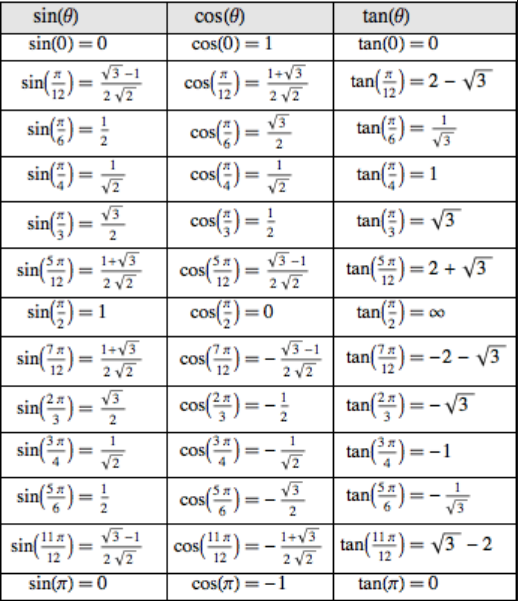
\includegraphics[width=0.4\linewidth]{p1Trig.png}}
	\subfigure{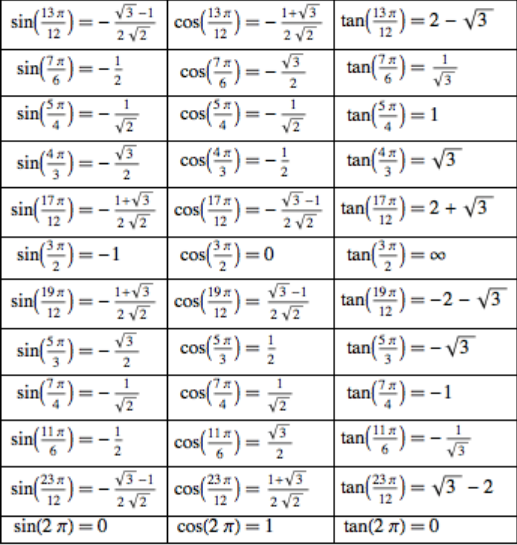
\includegraphics[width=0.41\linewidth]{p2Trig.png}}
\end{figure}

Dabei gelten die folgenden Gleichungen:

\begin{align*}
	\operatorname{exp}(iz) &= \cos (z) + i\sin(z)\\
	\cos(z) &= \cos(-z) & \sin (-z) &= - \sin(z) \\
	\sin (z) &= \frac{e^{iz} - e^{-iz}}{2i} & \cos (z) &= \frac{e^{iz} + e^{-iz}}{2}\\
	\sin(z+w) &= \sin(z) \cos(w) + \cos(z) \sin(w) \\
	\cos(z + w) &= \cos(z) \cos(w) - \sin(z) \sin(w)\\
	\cos(z) ^2 &+ \sin(z)^2 = 1\\
	\sin(x) - \sin(y) &=  2 \sin \left(\frac{x-y}{2}\right) \cos \left(\frac{x+y}{2}\right)\\
	\cos(x) - \cos(y) &= - 2 \sin \left(\frac{x-y}{2}\right) \sin \left(\frac{x+y}{2}\right)
\end{align*}

\textbf{Zeige $\sin(x)$ monton auf $[-\frac{\pi}{2}, \frac{\pi}{2}]$} Es gilt bekanntlich $\sin(x) - \sin(y) =  2 \sin \left(\frac{x-y}{2}\right) \cos \left(\frac{x+y}{2}\right) \geq 0$ wenn $-\frac{\pi}{2} \leq y < x \leq \frac{\pi}{2}$ womit auch $\frac{x-y}{2} \in (0,\frac{\pi}{2}]$ und $\frac{x+y}{2} \in (- \frac{\pi}{2}, \frac{\pi}{2})$

\TODO{anzuschliessen}



\subsection*{Hyperbolische Funktionen}
Es gilt:
\begin{align*}
	\cosh(x) &= \frac{e^x + e^{-x}}{2}\\
	\sinh(x) &= \frac{e^x - e^{-x}}{2}\\
	\tanh(x) &= \frac{\sinh(x)}{\cosh(x)} = \frac{e^x - e^{-x}}{e^x + e^{-x}}
\end{align*}
Dies gibt die folgenden Zusammenhänge:
\begin{align*}
	\cosh^2(x) - \sinh^2(x) &= 1\\
	\cosh(x) + \sinh(x) &= e^x\\
	\cosh(x) - \sinh(x) &= e^{-x}
\end{align*}

\newpage
% -------------------------- Ableitung --------------------------







\section{Ableitung}

\begin{method}{Häufungspunkt} 
	$x_0 \in \R$ ist ein Häufungspunkt der Menge $D$ falls $\forall \delta > 0$:
	$$(]x_0 - \delta, x_0 + \delta [ \setminus x_0) \cap D \not = \emptyset$$
\end{method}
\textbf{Beispiel (Häufungspunkt)} Sei $D = {0} \cup ] 1,2 [$, dann ist die Menge der Häufungspunkte von $D$, $D' = [1,2]$.


\begin{method}{Ableitung}
	Sei $D \subset \R$ , $f:D \to  \R$ und $x_0$ ein Häufungspunkt von $D$. $f$ ist in $x_0$ differenzierbar, falls der Grenzwert 
	$$ \lim\limits_{x \to x_0} \frac{f(x) -f(x_0)}{x-x_0}$$
	existiert. Ist dies der Fall, wird der Grenzwert mit $f'(x_0)$ bezeichnet.\\
	Alternativ nutzt man auch $x = x_0 + h$
	$$f'(x_0) = \lim\limits_{h \to 0} \frac{f(x_0 + h) - f(x_0)}{h}$$
\end{method}



\subsection*{Ableitungsregeln}
% to have more vertical space in the table.

{\renewcommand{\arraystretch}{1.5}
\begin{table}[]
	\begin{tabular}{@{} p{.25\textwidth} p{.3\textwidth} p{.45\textwidth} @{}}
		\toprule
		Funktion & Ableitung & Bemerkung / Regel\\ \midrule
		  $x$ & $1$ &   \\
		  $x^2$& $2x$ &   \\
		  $x^n$& $n\cdot x^{n-1}$ & $n \in \R$  \\
		  $\frac{1}{x} = x^{-1}$ & $- \frac{1}{x^2}$ & \\
		  $\sqrt{x} = x^{\frac{1}{2}}$ & $\frac{1}{2\sqrt{x}}$ & \\ 
		   $e^x$ & $e^x$ & \\
		  $a^x$ & $\ln(a) \cdot a^x$& \\
		  $\ln(x)$ & $\frac{1}{x}$ & \\ \midrule
		  $\sin(x)$ & $\cos(x)$ & \\
		  $\cos(x)$ & $- \sin(x)$ & \\ 
		  $\tan(x) = \frac{\sin(x)}{\cos(x)}$ & $\frac{1}{\cos^2(x)} = 1 + \tan^2(x)$ &\\
		  $\cot(x) = \frac{\cos(x)}{\sin(x)}$ & - $\frac{1}{\sin^2(x)}$ & \\ 
		  $\arcsin(x)$ & $\frac{1}{\sqrt{1 - x^2}}$ & $ \arcsin : [-1,1] \to [-\frac{\pi}{2},\frac{\pi}{2}]$\\
		  $\arccos(x)$ & $ - \frac{1}{\sqrt{1-x^2}}$ & $\arccos : [-1,1] \to [0, \pi]$\\
		  $\arctan(x)$ & $\frac{1}{1+x^2}$ & $\arctan:(-\infty, \infty) \to (- \frac{\pi}{2},\frac{\pi}{2})$\\
		  $\operatorname{arccot}(x)$ & $ - \frac{1}{1+x^2} $ & $\operatorname{arccot} : (-\infty, \infty) \to (0,\pi)$\\
		  \midrule
		  $\cosh(x)$ & $\sinh(x)$ &\\
		  $\sinh(x)$ & $\cosh(x)$ & \\
		  $\tanh(x)$ & $\frac{1}{\cosh^2(x)}$ & \\
		  $\operatorname{arsinh}(x)$ & $\frac{1}{\sqrt{1+x^2}}$ & $\forall x \in R$\\
		  $\operatorname{arcos}(x)$ & $\frac{1}{\sqrt{x^2 - 1}}$ & $\forall x \in (1, \infty)$\\		  $\operatorname{artanh}(x)$ & $\frac{1}{1-x^2}$ & $\forall x \in (-1,1)$\\
		  \midrule
		  $g(x) \cdot h(x)$ & $g(x) \cdot h'(x) + g'(x) \cdot h(x)$ & Produktregel\\
		  $\left(g(x)\right)^n$ & $n \cdot \left( g(x) \right)^{n-1} \cdot g'(x)$ & Potenzregel\\
		  $\frac{g(x)}{h(x)}$ & $\frac{ g'(x) \cdot h(x) - g(x)\cdot h'(x)}{\left(h(x)\right) ^2}$ & Quotientenregel\\
		  $h(g(x))$ & $h'(g(x)) \cdot g'(x)$ & Kettenregel\\
		  \bottomrule
	\end{tabular}
\end{table}
}




\begin{method}{Satz von Rolle}
	Sei $f: [a,b] \to \R$ stetig auf $(a,b)$ differenzierbar. Falls $f(a) = f(b)$, dann gibt es $\xi \in [a,b]$ mit $f'(\xi) = 0$
\end{method}
\textbf{Beweis (Satz von Rolle)} Aus dem Min-Max Satz folgt $\exists u,v \in [a,b]$ mit $f(u) \leq f(x) \leq f(v) \ \forall x \in [a,b]$. Falls einer der beiden in $(a,b)$ liegt nennen wir es $\xi$. Sonst gilt $f(a) = f(b)$ und dann $\xi = a$.


\begin{method}{Satz von Lagrange}
	Sei $f:[a,b] \to \R$ stetig mit $(a,b)$ differenzierbar. Dann gibt es $\xi \in (a,b)$ mit $$f(b) - f(a) = f'(\xi) (b-a)$$
	Dieser Satz ist auch bekannt als Mittelwertsatz. Die Aussage ist äquivalent zu: 
	$$\exists x \in (a,b) : \quad f'(c) = \frac{f(b) -f(a) }{b-a}$$
\end{method}
\textbf{Beispiele (Lagrange)}
\begin{itemize}
	\item \textit{Zeige $|\sin(a) - \sin(b)| \leq |b-a|$:} Es folgt direkt dass $\exists c$: $\frac{\sin(b)- \sin(a)}{b-a} = \cos(c)$. Es folgt: $\cos(c) (b-a) = \sin(b) - \sin(a)$. Da aber $\cos(c) \leq 1$ folgt:
	$|b-a| \geq |\sin(b) - \sin(a)|$.
	\item \textit{Beweise: falls $f'(x) = 0 \ \forall x$, dann ist $f(x)$ auf $[a,b]$ konstant:} Aus Lagrange folgt dass für $x_1,x_2\in (a,b)$ beliebig: $0 = \frac{f(x_2)-f(x_1)}{x_2-x_1}$ dies impliziert $f(x_1) = f(x_2)$ $\forall x_1,x_2 \in (a,b)$.
\end{itemize}



\begin{method}{Satz von Cauchy}
	Ein technischer Satz der für den Beweis von l'Hopital sowie Taylorapprox. gebraucht wird. Mit $g(x)=x$ hat man den Satz von Lagrange. \newline
Seien $f,g:[a,b]\to \R$ stetig und in $(a,b)$ differenzierbar. Dann gibt es $\xi \in (a,b)$ mit:
\begin{align*}
	g'(\xi)(f(b)-f(a)) &= f'(\xi)(g(b) - g(a))
\end{align*}
Falls zudem $g'(x) \not = 0$ $\forall x \in (a,b)$ folgt:
\begin{align*}
	g(a) \not = g(b)
\end{align*}
sowie:
\begin{align*}
	\frac{f(b) - f(a)}{g(b) - g(a)} &= \frac{f'(\xi)}{g'(\xi)}
\end{align*}
\end{method}


\subsection*{Konvexität}

\begin{method}{Konvex}
	$f : I \to \R$ ist konvex (auf I) falls für alle $x \leq y$ $x,y \in I$ und $\lambda \in [0,1]$
	\begin{align*}
	f(\lambda x + (1-\lambda)y) \leq \lambda f(x) + (1-\lambda)f(y)
	\end{align*}
	Zudem gilt für $x_0 < x< x_1$ in $I$:
	\begin{align*}
	 \frac{f(x) - f(x_0)}{x-x_0} \leq \frac{f(x_1) - f(x)}{x_1 - x}
	\end{align*}
	Man beweist dies indem man $x = (1-\lambda) x_0 + \lambda x_1$ wählt und somit $\lambda = \frac{x-x_0}{x_1 - x_0}$
\end{method}

\section*{Taylorapproximation}

\begin{method}{Taylorapproximation}
Sei $f\in C^m ([a,b])$ auf $(a,b)$ $m+1$ mal differenzierbar. Dann exisitert $\epsilon \in (a,b)$ mit 
\begin{align*}
	f(x) =& f(a) + f'(a)(x-a) + \ldots + \frac{1}{m!} f^{(m)} (a) (x-a)^m\\ &+ \frac{1}{(m+1)!} f^{(m+1)}(\xi) (x-a)^{m+1}
\end{align*} 
 \textbf{Beziehungsweise:}\\
	Sei $f:[a,b] \to \R$ stetig und in $(a,b)$ (n+1) mal differenzierbar. Für jedes $a<x\leq b$ gibt es $\xi \in (a,x)$ mit
	\begin{align*}
	f(x) &= \sum_{k=0}^n \frac{f^{(k)}(a)}{k!} (x-a)^k + \frac{f^{(n+1)(\xi)}}{(n+1)!} (x-a)^{n+1}
	\end{align*}

\end{method}

\textbf{Beispiel (Taylorapproximation)}
\begin{itemize}
	\item \textit{Finde $P_3 ^0 (x)$ von $f(x) = \sin(x)e^x$} Wir berechnen zuerst die Ableitungen:
	\begin{align*}
	    f(x) &= \sin(x)e^x & f(0) &= 0\\
		f'(x) &= e^x (\sin(x) + \cos(x)) & f'(0) &= 1\\
		f''(x) &= 2e^x \cos(x) & f''(0) &= 2\\
		f'''(x) &= 2e^x (\cos(x) - \sin(x)) & f'''(0) &=2 \\
		f''''(x) &= -4e^x\sin(x)
	\end{align*} 
	Dies gibt uns: 
	\begin{align*}
		P_3 ^0 (x) &= f(0) + f'(0)\cdot x + \frac{f''(x)}{2!} x^2 + \frac{f'''(x)}{3!}x^3\\
		&= 0 + 1 \cdot x + \frac{1}{2} \cdot 2 \cdot x^2 + 2 \frac{1}{3!}x^3\\
		&= x + x^2 + \frac{x^3}{3}
	\end{align*}
	Nun wollen wir den Fehler abschätzen:
	\begin{align*}
		|R_3 ^0 (x)| &= \left| \frac{-4e^c \sin(c)}{4!} x^4\right|\\
		&= \frac{e^c |\sin(c)|}{3!} x^4 \leq \frac{e^c}{3!} x^4 \quad \text{da }
	\end{align*}
	
	\item yet another example
	
\end{itemize}
\TODO{Definitionsraum von $x$ und $c$ ?????}

\TODO{add examples for taylor approximation}

\subsection*{Wichtige Taylorapproximationen um $x=0$}
\begin{itemize}
	\item $\boxed{\frac{1}{1-x}}$ Für alle $x \in (1,0)$ gilt:
	\begin{align*}
	{\frac{1}{1-x}} &= 1 + x + x^2 + x^3 + x^4 + \cdots \\
	&= \sum_{n=0}^{\infty} x^n
	\end{align*}	
	
	\item $\boxed{e^x}$ Für alle $x \in \R$ gilt:
	\begin{align*}
		e^x &= 1 + x + \frac{x^2}{2!} + \frac{x^3}{3!} + \frac{x^4}{4!}\\
		&= \sum_{n=0}^{\infty} \frac{x^n}{n!}
	\end{align*}
	
	\item $\boxed{\cos(x)}$ Für alle $x\in R$ gilt:
	\begin{align*}
	\cos(x) &= 1 - \frac{x^2}{2!} + \frac{x^4}{4!} - \frac{x^6}{6!} + \frac{x^8}{8!} - \cdots  \\
	&= \sum_{n=0}^{\infty} (-1)^n \frac{x^{2n}}{(2n)!}
	\end{align*}
	
	\item $\boxed{\sin(x)}$ Für alle $x\in R$ gilt:
	\begin{align*}
	\sin(x) &=  x - \frac{x^3}{3!} + \frac{x^5}{5!} - \frac{x^7}{7!} + \frac{x^9}{9!} - \cdots\\
	&= \sum_{n=0}^{\infty} (-1)^n \frac{x^{2n+1}}{(2n+1)!} = \sum_{n=1}^{\infty} (-1)^{(n-1)} \frac{x^{2n-1}}{(2n-1)!}
	\end{align*}

	\item $\boxed{\ln(1+x)}$ Für alle $x\in (-1,1]$ gilt:
	\begin{align*}
	\ln(x+1) &= x - \frac{x^2}{2} + \frac{x^3}{3} - \frac{x^4}{4} + \frac{x^5}{5}- \cdots \\
	&= \sum_{n=1}^{\infty} (-1)^{(n+1)} \frac{x^n}{n}
	\end{align*}

	\item $\boxed{\arctan(x)}$ Für alle $x\in [-1,1]$ gilt:
	\begin{align*}
	\l\arctan(x) &= x - \frac{x^3}{3} + \frac{x^5}{5} - \frac{x^7}{7} + \frac{x^9}{9} - \cdots \\
	&= \sum_{n=0}^{\infty} (-1)^n \frac{x^{2n+1}}{2n+1}
	\end{align*}

	
\end{itemize}







% -------------------------- Integration --------------------------


\section{Integration}


% -------------------------- Sonstiges --------------------------









\section{Sonstiges}
\begin{method}{Binomialsatz}
	$\forall x,y \in \mathbb{C}$, $n \geq 1$ gilt:
	$$(x+y)^n = \sum_{k=0}^{n} \binom{n}{k}x^k y^{n-k}$$
\end{method}


\newpage

\end{multicols}
\end{document}
